\subsection{Gráfico}

\begin{example}
    Considere as funções logarítmicas tais que $f(x) = \log_2 x$ e $g(x) = \log_{\frac 1 2} x$. Os gráficos de $f$ e $g$ são apresentados abaixo.
    \begin{figure}[H]
        \centering
        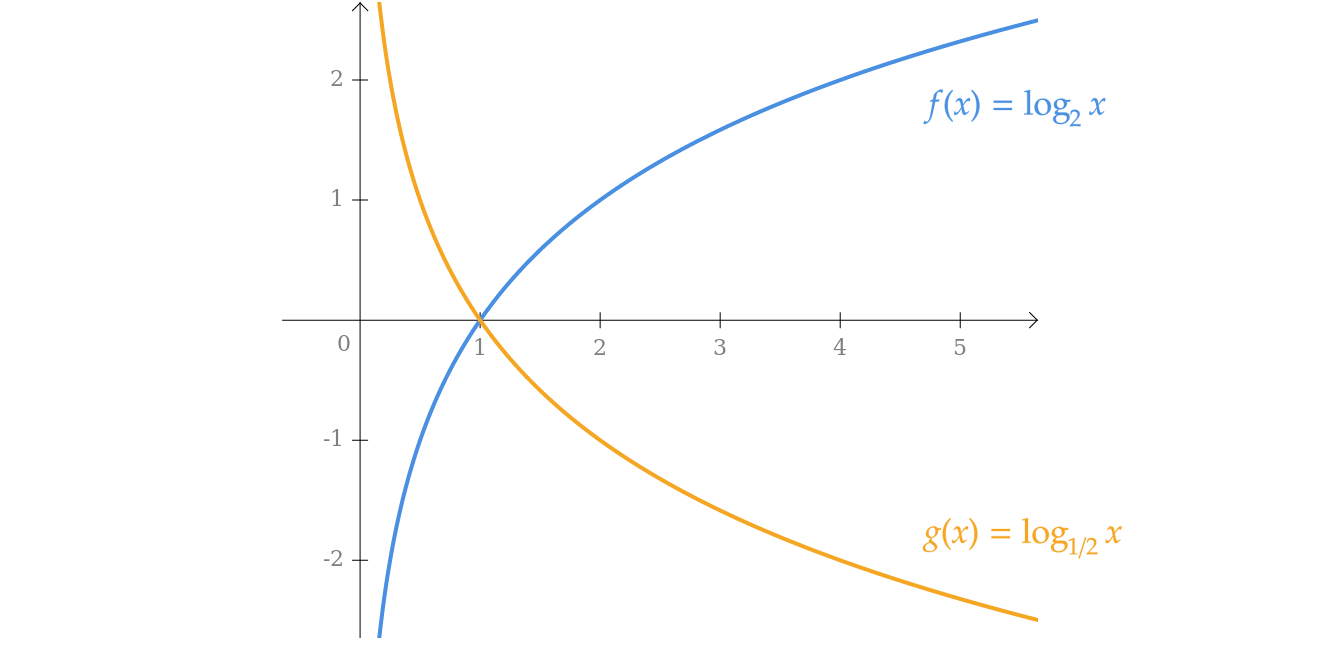
\includegraphics[scale=0.30]{\imgdirfromsection/grafico-logaritmica.png}
        \caption{Gráficos das funções $f$ e $g$.}
        \label{img:grafico-logaritmica}
    \end{figure}
\end{example}

Qual a relação entre os gráficos dessas funções?

\begin{solution}
    Seja $f(x) = \log_2 x$. Teremos:
    \[
        g(x) = \log_{\frac 1 2}{x}
        = \frac{\log_2 x}{\log_2 {\frac 1 2}}
        = \frac{\log_2 x}{\log_2 \prn{2^{-1}}}
        = \frac{\log_2 x}{-1\cdot\log_2 2}
        = -\log_2 x
        = -f(x)
    \]
    Assim, o gráfico de $g(x)$ é, simplesmente, uma reflexão do gráfico de $f(x)$.
\end{solution}

\begin{remark}
    Já vimos que o crescimento exponencial supera o de qualquer polinômio. Por ser a inversa da função exponencial, a função logarítmica possui um crescimento muito lento. Mesmo assim, a função logarítmica é ilimitada superiormente. Compare os gráficos abaixo:
\end{remark}

\begin{onlineact}
    \khan{https://pt.khanacademy.org/math/algebra2/exponential-and-logarithmic-functions/graphs-of-logarithmic-functions/e/graphs-of-exponentials-and-logarithms}{Gráficos de Funções Logarítmicas}
\end{onlineact}